Im Rahmen dieser Arbeit wurden zwei Systeme zur Erkennung von Hindernissen in Echtzeit entwickelt. Diese richten sich nach den in Kapitel REF erläuterten Algorithmen und Konzepten. Anhand dieser ist es möglich aus den beiden Bildern des Stereo Systems für jeden Frame die Disparity Map zu berechnen, welche im Anschluss daran in mehreren Schritten zunächst so angepasst wird, dass nicht verwertbare Bereiche der Tiefenkarte entfernt werden (siehe REF preprocessing). Dies reduziert die Anzahl der zur Erkennung zu verarbeitenden Punkte und somit die Rechenzeit.\\

\noindent
Im folgenden Kapitel werden beide Methoden detailliert beleuchtet. Zu Beginn wird die zugrunde liegende Klassenstruktur beschrieben. In Abschnitt \ref{sec:mean_disparity_detection} die \emph{Mean Disparity Detection} erläutert, wobei auf das grundlegende Konzept sowie den Algorithmus zur Erkennung selber eingegangen wird. Selbiges gilt für die \emph{Samplepoint Detection} in Abschnitt \ref{sec:samplepoint_detection}.


\begin{figure}[h]
	\begin{center}
	    %TODO: change Samplepoint Detection mImageCenter to private
	    %TODO: add Subimage Stuff to MeanDisparityDetection
		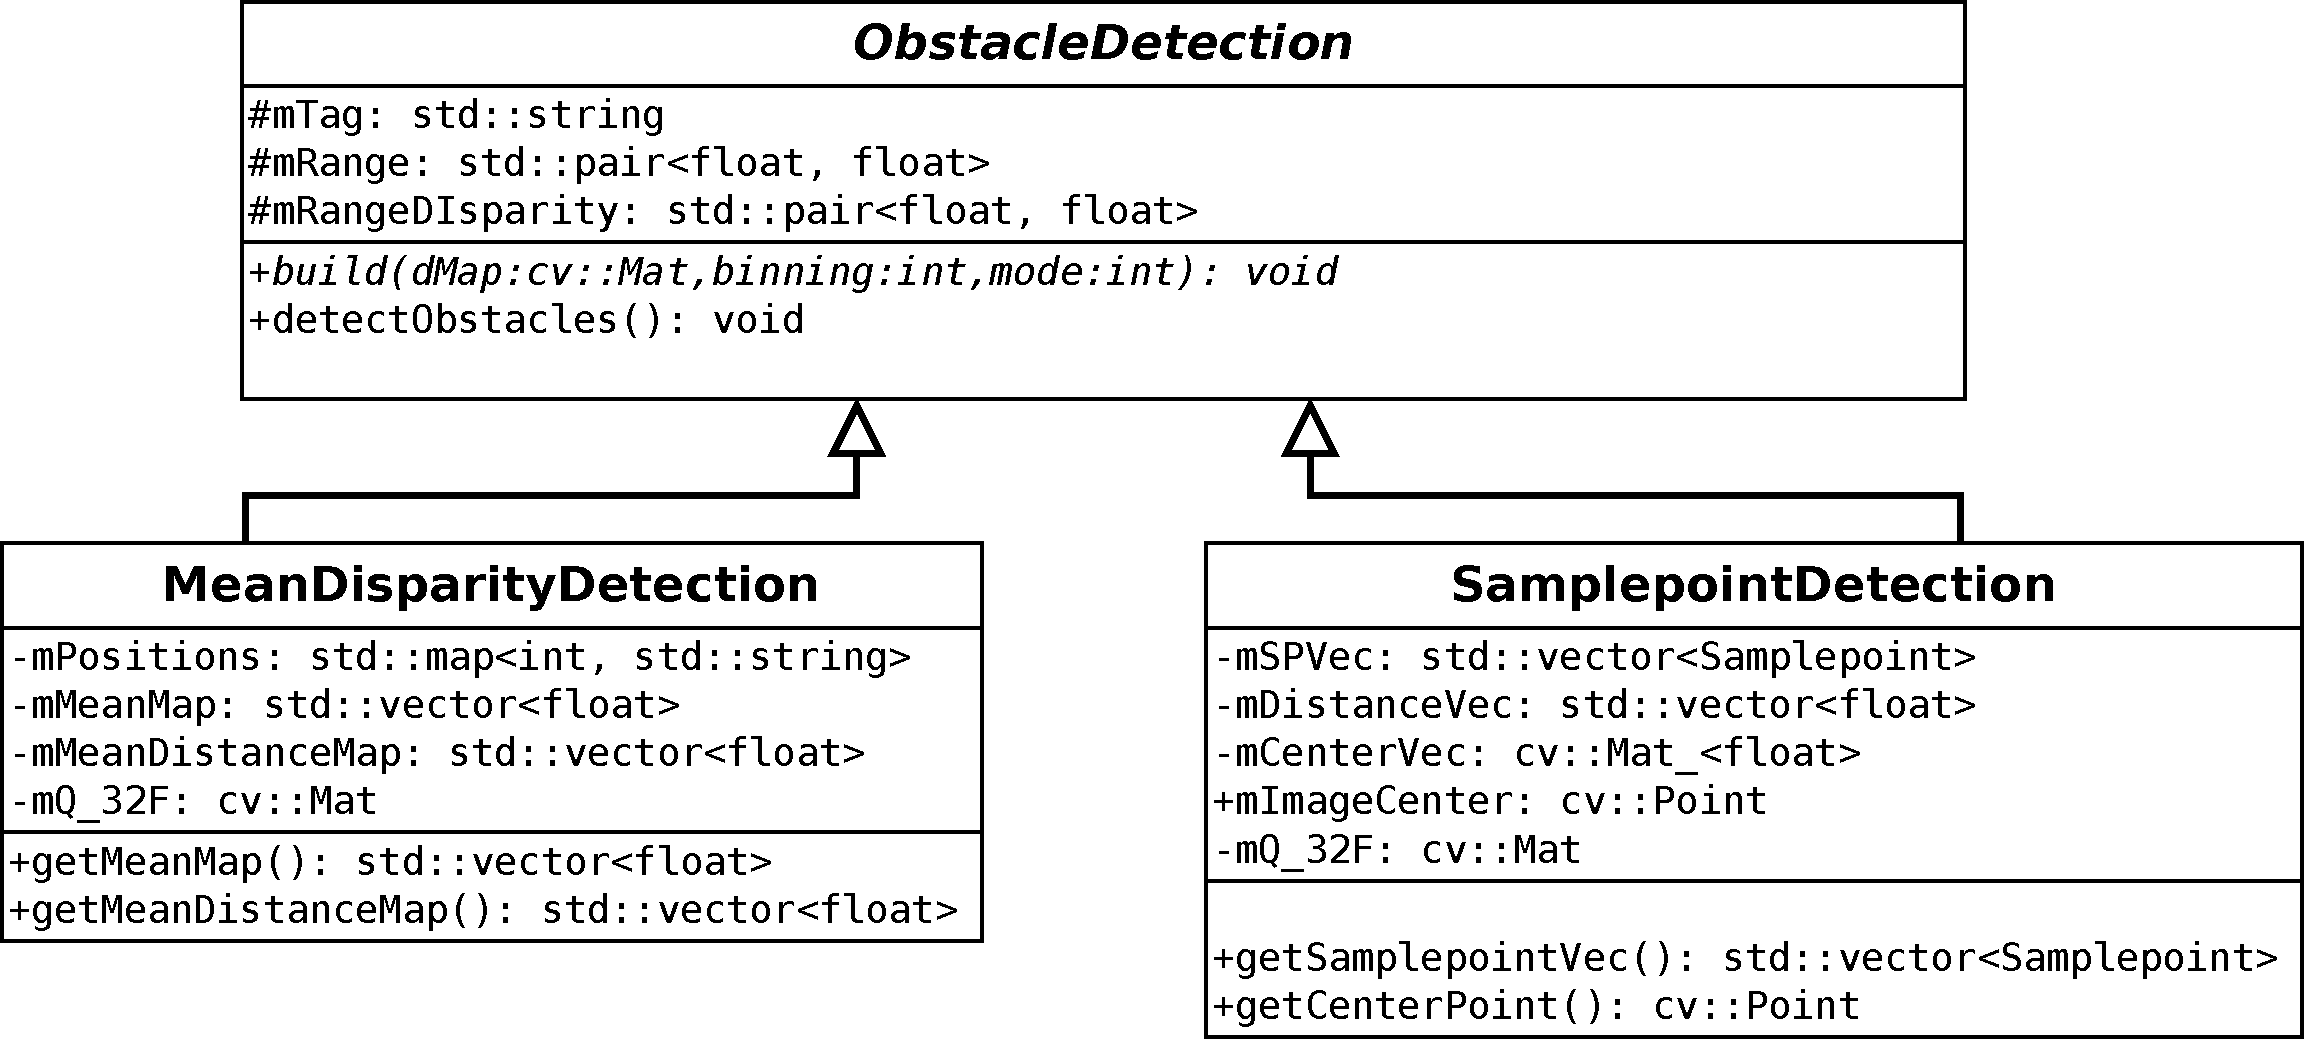
\includegraphics[width=13cm]{img/obstacle_detection_structure.pdf}
	\end{center}
	\caption{Klassenstruktur der Hinderniserkennung}
	\label{fig:obstacle_detection_structure}
\end{figure}



% ---------------------- section -----------------------
\section{Mean Disparity Detection}
\label{sec:mean_disparity_detection}

\begin{algorithm}[h]
\caption{Berechnung des Disparity Medians}
\label{alg:mean_disparity_calculation}
\begin{algorithmic}[1]
    \Procedure{CalcMeanDisparity}{$submatrix$}
        \State $elements_{number} \gets 0$
        \State $elements_{sum} \gets 0 $
        \For{$value$ in $submatrix$}
            \If{$value > 0$}
                \State $elements_{sum} \gets elements_{sum} + value$
                \State $elements_{number} \gets elements_{number} + 1$
            \EndIf
        \EndFor
        \State \textbf{return} $elements_{sum} / elements_{number}$
    \EndProcedure
\end{algorithmic}  
\end{algorithm}

% ---------------------- section -----------------------
\section{Samplepoint Detection}
\label{sec:samplepoint_detection}

